\begin{center}
	\Huge
	Grænseværdier
\end{center}

\section*{Grænseværdier}
\stepcounter{section}

Grænseværdibegrebet er et begreb, vi bruger, når vi sådan lidt løst beskrevet gerne vil vide, hvad der sker med  funktionsværdien, når vores $x$-værdier enten bliver meget positive, meget negative eller kommer meget tæt på en anden fastholdt værdi $x_0$. 

Det er væsentligt nemmere at eksemplificere bestemmelsen af grænseværdier end det er at definere dem præcist. Derfor betragter vi indledningsvist en række eksempler.

\begin{exa}
	Funktionen $f: \mathbb{R}_{>0} \to \mathbb{R}$ givet ved
	\begin{align*}
		f(x) = \frac{1}{x}
	\end{align*}
	kan ses tegnet på Figur \ref{fig:grænse}.
	\begin{figure}[H]
	\centering
	\begin{tikzpicture}
	\begin{axis}[
		axis lines = center, 
		xmin = -0.5, xmax = 5, 
		ymin = -0.5, ymax = 5,
		xlabel = $x$, ylabel = $y$,
	]
		\addplot[color = teal, thick, domain = 0.1:5, samples = 300] {1/x};
	\end{axis}
	\end{tikzpicture}
	\caption{Graf for funktionen $f$.}
	\label{fig:grænse}
	\end{figure}
	Lader vi $x$ vokse, så vil funktionsværdien for $f$ komme tættere og tættere på nul, da afstanden fra 
	grafen for $f$ og $x$-aksen bliver mindre og mindre. Vi kan også observere dette ved at anvende 
	funktionsforskriften. Det er klart, at når vi gør $x$ større, så vil 
	\begin{align*}
		f(x) = \frac{1}{x}
	\end{align*}
	blive mindre og mindre. Vi siger i dette tilfælde, at $f$ går mod $0$ når $x$ går mod $\infty$. Dette kan 
	skrives på to måder. Enten ved at skrive
	\begin{align*}
		f(x) \to 0 \textnormal{ når } x \to \infty 
	\end{align*}
	eller mere typisk
	\begin{align*}
		\lim_{x \to \infty} f(x) = 0. 
	\end{align*}
	Dette læses som \textit{grænseværdien for f når x går mod uendelig er lig 0}.
	
	Betragter vi igen grafen på Figur \ref{fig:grænse} kan vi tilsvarende se, at 
	\begin{align*}
		\lim_{x \to 0} = \infty
	\end{align*}
	under den antagelse, at $f$ kun er defineret for positive $x$. 
\end{exa}
\begin{exa}
	Vi betragter nu samme funktion $g: \mathbb{R} \to \mathbb{R}$ givet ved
	\begin{align*}
		g(x) = \frac{1}{x}
	\end{align*}	 
	men nu med hele $\mathbb{R}$ som	definitionsområde. Vi kan se grafen for denne på Figur \ref{fig:grænse2}
	\begin{figure}[H]
	\centering
	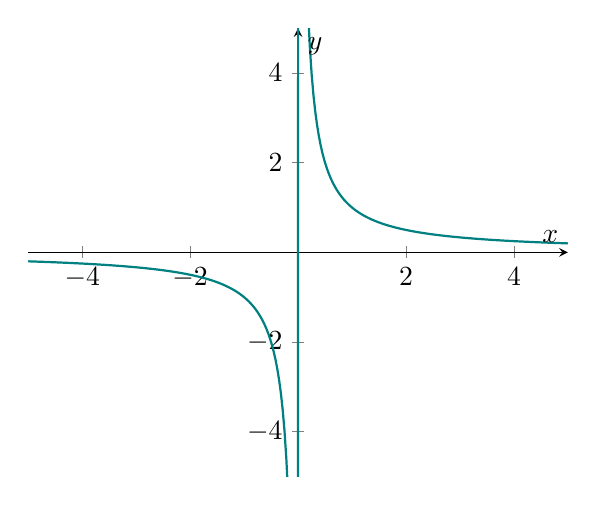
\begin{tikzpicture}
	\begin{axis}[
		axis lines = center, 
		xmin = -5, xmax = 5, 
		ymin = -5, ymax = 5,
		xlabel = $x$, ylabel = $y$,
	]
		\addplot[color = teal, thick, domain = -5:5, samples = 300] {1/x};
	\end{axis}
	\end{tikzpicture}
	\caption{Graf for funktionen $g$.}
	\label{fig:grænse2}
	\end{figure}
	Vi kan tilsvarende her se, at 
	\begin{align*}
		\lim_{x \to \infty} g(x) = 0
	\end{align*}
	og 
	\begin{align*}
		\lim_{x \to -\infty} g(x) = 0.
	\end{align*}
	Der opstår dog et problem, når vi prøver at bestemme grænseværdien når $x \to 0$. Lader vi $x$ nærme sig 0
	fra højre, så får vi grænseværdien $\infty$. 
	Dette skrives som 
	\begin{align*}
		\lim_{x \to 0^+} = \infty 	
	\end{align*}		
	 Lader vi derimod $x$ nærme sig 0 fra venstre, så får
	vi grænseværdien $-\infty$. Dette skrives som
	\begin{align*}
		\lim_{x \to 0^{-}} = -\infty.
	\end{align*}
	I tilfældet af at grænseværdien ikke er den samme fra venstre og højre, så siges grænseværdien ikke at 
	eksistere.
\end{exa}
Vi giver nu denne lidt upræcise definition af grænseværdien for en funktion.
\begin{defn}[Grænseværdi]
	For en funktion $f:\mathbb{R} \to \mathbb{R}$ siges grænseværdien for $f$ i punktet $x_0$ at eksistere, 
	hvis grænseværdierne fra højre og venstre i punktet er ens, altså at
	\begin{align*}
		\lim_{x \to x_0^+}f(x) = \lim_{x \to x_0^-}f(x).
	\end{align*}
	Grænseværdien betegnes i dette tilfælde
	\begin{align*}
		\lim_{x \to x_0}f(x).
	\end{align*}
\end{defn}
\begin{exa}
	Vi kan sagtens have grænseværdier, hvor der ikke indgår uendelighed. Vi betragter nu funktionen 
	$h:\mathbb{R} \to \mathbb{R}$ givet ved
	\begin{align*}
		h(x) = 
		\begin{cases}
		-x^2 + 6, \ &\textnormal{hvis } x < 2, \\
		5, &\textnormal{hvis } x = 2, \\
		3x - 4, &\textnormal{hvis } x > 2. 
		\end{cases}
	\end{align*}
	Vi kan se grafen for $h$ på Figur \ref{fig:grænse3}.
	\begin{figure}[H]
	\centering
	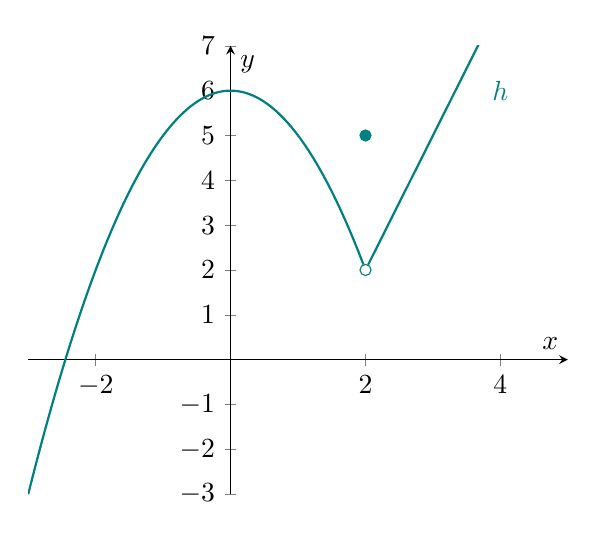
\begin{tikzpicture}
	\begin{axis}[
		axis lines = center, 
		xmin = -3, xmax = 5, 
		ymin = -3, ymax = 7,
		ytick = {-3,-2,...,6,7},
		xlabel = $x$, ylabel = $y$,
	]
		\addplot[color = teal, thick, domain = -3:2, samples = 100] {-x^2 + 6};
		\addplot[color = teal, thick, domain = 2:5, samples = 100] {3*x -4};
		\filldraw[color = teal] (axis cs: 2,5) circle (2pt);
		\filldraw[color = white] (axis cs: 2,2) circle (2pt);
		\draw[color = teal] (axis cs: 2,2) circle (2pt);
		\node[color = teal] at (axis cs: 4,6) {$h$};
	\end{axis}
	\end{tikzpicture}
	\caption{Graf for funktionen $h$.}
	\label{fig:grænse3}
	\end{figure}
	For $h$ har vi grænseværdierne fra højre og venstre givet ved 
	\begin{align*}
		\lim_{x \to 2^+} h(x) = 2
	\end{align*}
	samt 
	\begin{align*}
		\lim_{x \to 2^-}h(x) = 2,
	\end{align*}
	så grænseværdien for $h$ for $x \to 2$ eksisterer og er lig $2$.
\end{exa}
Vi kan også være ude for at skulle bestemme grænseværdier for funktioner, hvor vi ikke kender grafen for funktionen. 
\begin{exa}
	For funktion $f$ givet ved
	\begin{align*}
		f(x) = \frac{x^2 + x}{x + 1}
	\end{align*}
	er det ikke oplagt, hvad grænseværdien
	\begin{align*}
		\lim_{x \to -1}f(x)
	\end{align*}
	skal give, da vi både i nævner og tæller får $0$, hvis vi blot indsætter tallet. 
	Dette kaldes for et \textit{0/0-udtryk} eller en \textit{ubestemt form}. Derfor kræver evalueringen
	af denne grænseværdi lidt omskrivning. Vi kan skrive
	\begin{align*}
		f(x) = \frac{x^2 + x}{x + 1} = \frac{x(x+1)}{x+1} = x,
	\end{align*}
	og det er nu lettere at evaluere grænseværdien, da vi så får
	\begin{align*}
		\lim_{x \to -1}f(x) =\lim_{x \to -1}x = -1
	\end{align*}
\end{exa}

\newpage
\subsection*{Opgave 1}
Bestem følgende grænseværdier

\begin{align*}
	&1) \ \lim_{x \to 3} 2x + 4 &  &2) \ \lim_{x \to 0} 4x^2 -4x + 2 \\
	&3) \ \lim_{x \to 0} \sin(x) + 2x &  &4) \ \lim_{x \to 6} \sqrt{x - 2} - 5x
\end{align*}

\subsection*{Opgave 2}
Bestem følgende grænseværdier, der giver 0/0-udtryk. (Vink: Det kan være en fordel at bruge kvadratsætninger til nogle af udtrykkene). Tegn evt. graferne i Maple for at kontrollere, om I har fundet den korrekte grænseværdi.

\begin{align*}
	&1) \ \lim_{x \to 0} \frac{2x^2+4x}{x} & &2) \ \lim_{x \to 2} \frac{x^2 - 4}{x - 2} \\
	&3) \ \lim_{x \to -3} \frac{x^2 - 9}{x+3} & &4) \ \lim_{x \to 4} \frac{2x^2 - 32}{x - 4} \\
	&5) \ \lim_{x \to -1} \frac{x^2 + 2x + 1}{x+1} & &6) \ \lim_{x \to -3} \frac{x^2+x-6}{x+3} \\
\end{align*}


\subsection*{Opgave 3}
Bestem følgende grænseværdier, hvor $x \to \infty$ eller $x \to -\infty$. 
(Vink: Det kan være en fordel at dividere både tæller og nævner med den højeste potens af $x$).
Tegn evt. graferne i Maple for at kontrollere, om I har fundet den korrekte grænseværdi.

\begin{align*}
	&1) \ \lim_{x \to \infty} \frac{2x^2 + 4}{x^2 + 1} & &2) \ \lim_{x \to -\infty} \frac{3x^3 - 2}{5x^3 + 4} \\
	&3) \ \lim_{x \to \infty} \frac{4x^4 + 2}{2x^5 - 3} & &4) \ \lim_{x \to -\infty} \frac{5x^6 - 1}{3x^4 + 7} \\
	&5) \ \lim_{x \to \infty} \frac{-5x^7 + 2x^4 -3x + 1}{10x^7	-3x^3-10x+2} & 
	&6) \ \lim_{x \to -\infty} \frac{9x^5 - 11x^4}{3x^5 + 4x^2 -2x + 3} \\
\end{align*}
\newpage


\subsection*{Opgave 4}
Grafen for funktionen $f$ kan ses på Figur \ref{fig:kont1}.

\begin{figure}[H]
	\centering
	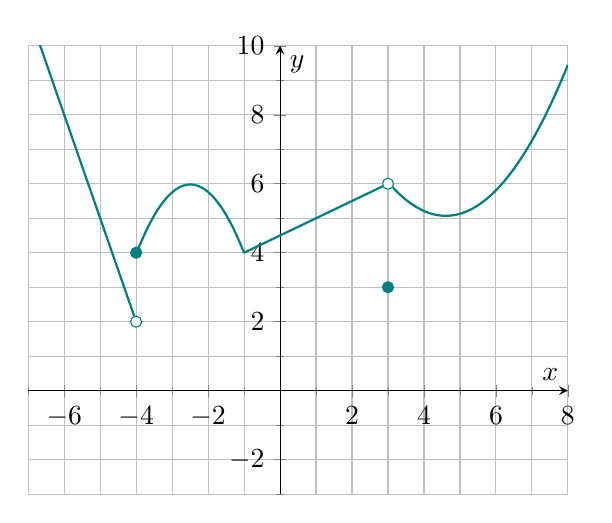
\begin{tikzpicture}
	\begin{axis}[
		axis lines = center, 
		xmin = -7, xmax = 8, 
		ymin = -3, ymax = 10,
		xlabel = $x$, ylabel = $y$,
		minor tick num = 1,
		grid = both,
	]
		\addplot[color = teal, thick, domain = -7:-4] {-3*x - 10};
		\addplot[color = teal, thick, domain = -4:-1, samples = 100] {-0.89*x^2-4.44*x+0.44};
		\addplot[color = teal, thick, domain = -1:3, samples = 100] {0.5*x + 4.5};
		\addplot[color = teal, thick, domain = 3:8, samples = 100] {0.38*x^2-3.5*x + 13.13};
		%Circle1
		\filldraw[color = white] (axis cs: -4,2) circle (2pt);
		\draw[color = teal] (axis cs: -4,2) circle (2pt);
		%Circle2
		\filldraw[color = teal] (axis cs: -4,4) circle (2pt);
		%Circle3
		\filldraw[color = white] (axis cs: 3,6) circle (2pt);
		\draw[color = teal] (axis cs: 3,6) circle (2pt);
		%Circle4
		\filldraw[color = teal] (axis cs: 3,3) circle (2pt);
	\end{axis}
	\end{tikzpicture}
	\caption{Graf for funktionen $f$.}
	\label{fig:kont1}
\end{figure}
\begin{enumerate}[label=\roman*)]
	\item Bestem tallene $f(-4)$, $f(-1)$, $f(1)$ og $f(3)$. 
	\item Bestem følgende grænseværdier
	\begin{align*}
		&1) \ \lim_{x \to -4^-}f(x) &   &2) \ \lim_{x \to -4^+}f(x) \\
		&3) \ \lim_{x \to -1^-}f(x) &   &4) \ \lim_{x \to -1^+}f(x) \\
		&5) \ \lim_{x \to 3^-}f(x) &   &6) \ \lim_{x \to 3^+}f(x) \\
	\end{align*}
	\item I hvilke af punkterne $-4$, $-1$ og $3$ eksisterer grænseværdien?
\end{enumerate}

\newpage

\subsection*{Opgave 5}
Grafen for funktionen $g$ kan ses på Figur \ref{fig:kont2}.
\begin{figure}[H]
	\centering
	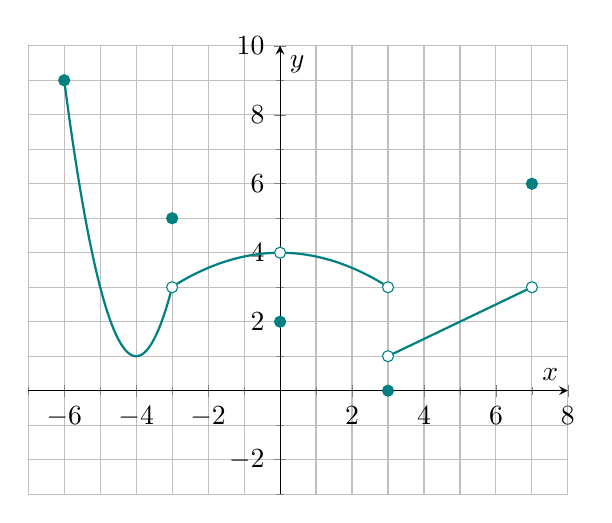
\begin{tikzpicture}
	\begin{axis}[
		axis lines = center, 
		xmin = -7, xmax = 8, 
		ymin = -3, ymax = 10,
		xlabel = $x$, ylabel = $y$,
		minor tick num = 1,
		grid = both,
	]
		\addplot[color = teal, thick, domain = -6:-3, samples = 100] {2*x^2+16*x+33};
		\addplot[color = teal, thick, domain = -3:3, samples = 100] {-0.11*x^2 + 4};
		\addplot[color = teal, thick, domain = 3:7, samples = 100] {0.5*x-0.5};
		\filldraw[color = teal] (axis cs: -6,9) circle (2pt);		
		\filldraw[color = white] (axis cs: -3,3) circle (2pt);
		\draw[color = teal] (axis cs: -3,3) circle (2pt);
		\filldraw[color = teal] (axis cs: -3,5) circle (2pt);
		\filldraw[color = white] (axis cs: 0,4) circle (2pt);
		\draw[color = teal] (axis cs: 0,4) circle (2pt);		
		\filldraw[color = teal] (axis cs: 0,2) circle (2pt);
		\filldraw[color = white] (axis cs: 3,3) circle (2pt);
		\draw[color = teal] (axis cs: 3,3) circle (2pt);		
		\filldraw[color = white] (axis cs: 3,1) circle (2pt);
		\draw[color = teal] (axis cs: 3,1) circle (2pt);
		\filldraw[color = teal] (axis cs: 3,0) circle (2pt);
		\filldraw[color = white] (axis cs: 7,3) circle (2pt);
		\draw[color = teal] (axis cs: 7,3) circle (2pt);
		\filldraw[color = teal] (axis cs: 7,6) circle (2pt);		
	\end{axis}
	\end{tikzpicture}
	\caption{Graf for funktionen $g$.}
	\label{fig:kont2}
\end{figure}
\begin{enumerate}[label=\roman*)]
	\item Bestem tallene $g(-6)$, $g(-3)$, $g(0)$, $g(3)$ og $g(7)$
	\item Bestem grænseværdierne i punkterne $-6$, $-3$, $0$, $3$ og $7$, hvis de eksisterer.
\end{enumerate}

\newpage

\subsection*{Opgave 6}
Har vi et udtryk $\sqrt{x} + a$, så kalder vi udtrykket $\sqrt{x} - a$ for det konjugerede udtryk. Dette kan ofte bruges til at bestemme grænseværdier med 0/0-udtryk. 
\begin{enumerate}[label=\roman*)]
	\item Vi ønsker at bestemme grænseværdien
	\begin{align*}
		\lim_{x \to 4} \frac{\sqrt{x}-2}{x-4}.
	\end{align*}
	Forlæng først brøken med det konjugerede udtryk $\sqrt{x}+2$. 
	\item Gang udtrykket i tælleren sammen, men lad parenteserne i nævneren stå.
	\item Forkort udtrykket og evaluér grænseværdien
\end{enumerate}

Bestem følgende grænseværdier, der giver 0/0-udtryk ved at forlænge med det konjugerede udtryk. 

\begin{align*}
	&1) \ \lim_{x \to 9} \frac{\sqrt{x}-3}{x-9}    & &2) \ \lim_{x\to 3}\frac{\sqrt{x+1} - 2}{x-3}  \\
	&3) \ \lim_{x \to 0} \frac{\sqrt{x + 1} - 1}{x}  & &4) \ \lim_{x \to 4} \frac{\sqrt{x^2 -12}-2}{x-4}  \\
\end{align*}

\newpage